\section{Comparison with Chinchilla Scaling Law}
\label{sec:comparison}

\subsection{Reduction to Chinchilla Scaling Law}
Our scaling law equation can predict the full loss curve across any given LRS. In this section, we show    
that our equation has no contradiction with traditional scaling laws, and it is a generalized form of the Chinchilla scaling law~\citep{hoffmann2022training}. Specifically, all the final loss values for different total training steps following our equation should also follow a power-law relationship. We prove this by dividing two conditions: (1) constant LRS, and (2) other LRS.


\noindent \textbf{Constant LRS.} In the case of a constant LRS, the annealing area $S_2$ is always zero and the forward area $S_1 = \eta_{max} \cdot s$, where $s$ is the step, and $\eta_{max}$ is the constant maximal LR. Thus, the whole loss curve formula becomes:
% $L(s) = L_0 + (A\cdot \eta_{max}^{-\alpha})  \cdot s^{-\alpha} =  L_0 + A^{\prime} \cdot s^{-\alpha}$,
\begin{equation}
L(s) = L_0 + (A\cdot \eta_{max}^{-\alpha})  \cdot s^{-\alpha} =  L_0 + A^{\prime} \cdot s^{-\alpha} 
\end{equation}
which aligns with the Chinchilla scaling law equation. 


\noindent \textbf{Other LRS.} For non-constant LRS, we use a statistical approach to show that our equation can be reduced to the Chinchilla scaling law. 
Specifically, we verify whether the Chinchilla scaling law adequately fits the endpoints of loss curves predicted by our equation.
The parameter tuple of our equation is $(L_{0}, A, C, \alpha)$. We then randomly sample 1000 sets of parameter tuples from some uniform distributions:
$L_0\sim U(1,3)$, $A\sim U(0.3,0.5)$, $C\sim U(0.2,0.6)$,  $\alpha\sim U(-0.6,-0.4)$.
Each parameter tuple could be seen as the fitting result of a distinct set of experimental setups~\footnote{It's worth noting that some of these sampled parameter tuples might not be reasonable or likely to be observed in real experiments, but we choose to keep them nonetheless.}. (e.g. dataset, batch size, model size, etc.).
For each generated parameter tuple, we apply our equation to predict the final loss of different total training steps on two LRS including cosine and WSD (10\% annealing ratio), 
ranging from 5K to 60K steps. 
The predicted loss values on final steps are used to fit the chinchilla equation. 
The fitting results are shown in Fig.~\ref{fig:phe-reduction}.

\begin{table}[htbp]
\begin{center}
\caption{Mean and standard deviation of $R^2$, as well as the mean Huber loss of 1,000 randomly
generated parameter tuples.}
\label{tab:reduction}
\begin{tabular}{lccc}
\toprule
\textbf{LR Scheduler} & \textbf{mean}($R^2$) $\uparrow$ & \textbf{std}($R^2$) $\downarrow$ & \textbf{Huber Loss} $\downarrow$ \\
\midrule
Cosine         &0.972 &0.056 & 0.00017 \\
WSD             &0.979  &0.053 & 0.00013 \\
\bottomrule
\end{tabular}
\end{center}
\end{table}


\begin{figure}[tbp]
    \centering
    \begin{subfigure}[b]{0.48\textwidth}
        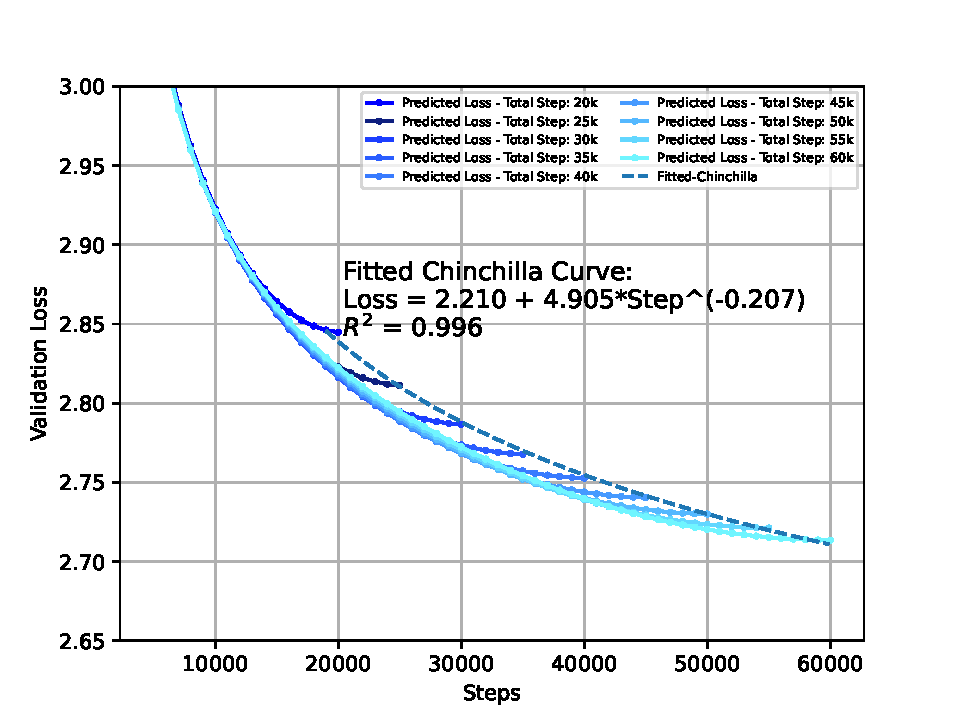
\includegraphics[width=\textwidth]{images/reduce_cosine.pdf}
        \caption{The predicted loss of different total steps with cosine LRS and the fitted chinchilla curve.}
    \end{subfigure}
    \hfill
    \begin{subfigure}[b]{0.48\textwidth}
        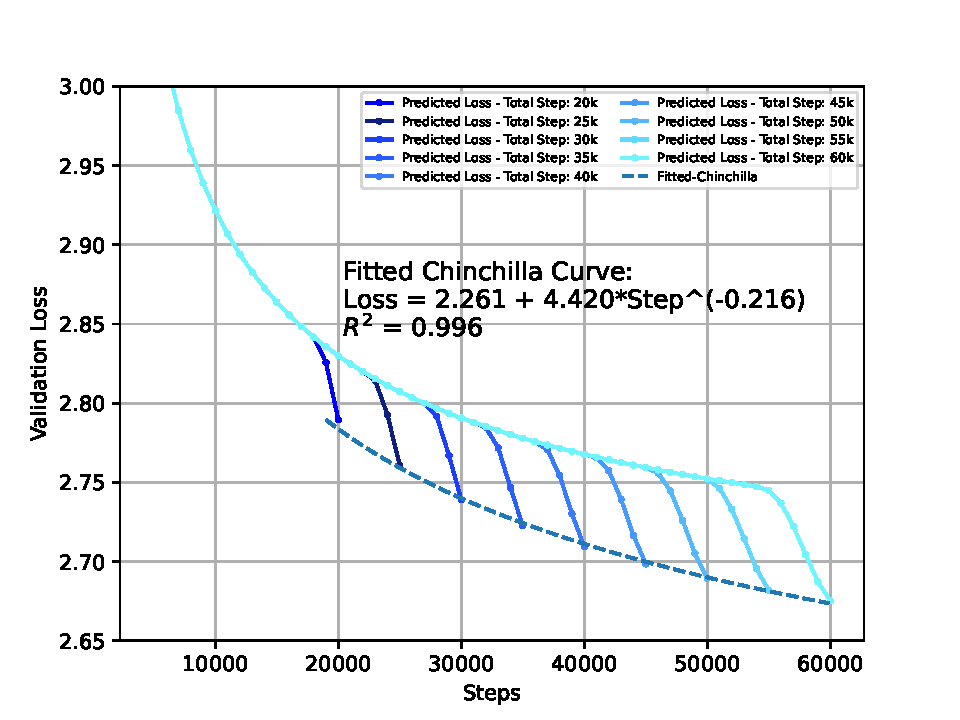
\includegraphics[width=\textwidth]{images/reduce_wsd.pdf}
        \caption{The predicted loss of different total steps with WSD LRS and the fitted chinchilla curve.}
    \end{subfigure}
    \caption{The Chinchilla scaling law equation fits well on the final validation losses predicted by our formulation, taking cosine LRS (on the left) and WSD LRS (on the right) as examples.}
\label{fig:phe-reduction}
\end{figure}

Each parameter tuple represents a synthetic fitting result corresponding to a distinct set of experimental setups (e.g. dataset, model size, etc.).
For each sampled parameter tuple, we apply our equation to predict the final loss for different total training steps with both cosine and WSD LRS, and then employ the predicted losses to fit the Chinchilla scaling law.
We calculate the mean and standard deviation of $R^{2}$ values for each fit. 
The results in Table~\ref{tab:reduction} demonstrate that Chinchilla scaling law fits well on the data predicted by our scaling law equation. Thus, our equation can be considered a generalization that can be reduced to the Chinchilla scaling law. 

\subsection{Scaling Law Fitting and Prediction Democratization}

Our scaling law equation allows us to utilize all loss values from a full loss curve during training, while traditional scaling laws can only collect a single data point from the full loss curve. This feature allows us to fit scaling laws with much less cost.
For a direct comparison, we compare the computational efficiency of our approach and the Chinchilla scaling law~\citep{hoffmann2022training}.
Specifically, we assume and evaluate the computational cost of obtaining 100 fitting points for each scaling law equation with an step interval of $K$: 
% \begin{itemize}
%     \item Fitting the \textbf{Chinchilla scaling law equation with the cosine LRS} requires a total number of parameter updates of $1K + 2K + 3K + \dots + 100K = 5050K$;
%     \item Fitting the \textbf{Chinchilla scaling law equation with the WSD LRS} requires a total number of parameter updates of $(1K + 2K + 3K + \dots + 100K)r + 100K(1-r) = (100 + 4950r)K$, in which $r$ is the annealing ratio for the WSD LRS;
%     \item Fitting \textbf{our scaling law equation} only need one training curve with a moderate number of parameter updates, such as one curve under the cosin LRS with $50K$ training steps. Further, the number of loss values we can get for fitting our equation is far more than $100$. Note that more fitting points generally achieve more accurate fitting results. Our equation can also utilize loss curves from various different LRS (e.g. $20K$ constant + $30K$ cosine).
% \end{itemize}

\begin{itemize}
    \item Adopting Chinchilla scaling law, typical cosine LRS requires total steps of at least $1K + 2K + 3K + \cdots + 100K = 5050K$;
    \item Adopting Chinchilla scaling law, WSD LRS (notating annealing ratio as $r$) requires total steps of at least $(1K + 2K + 3K + \cdots + 100K)r + 100K(1-r) = (100 + 4950r)K$.
    \item Adopting our scaling law, all we need is only one or two training curves with moderate total steps, such as one curve with $50K$ steps under cosine LRS. Further, the number of loss values we can get for fitting our equation is far more than $100$. Note that more fitting points generally achieve more accurate fitting results. Our equation can also utilize loss curves from various different LRS (e.g. $20K$ constant + $30K$ cosine)
\end{itemize}


\begin{table}[tbp]
\begin{center}
\caption{The comparison of computational cost for fitting different scaling law equations.}
\label{tab:green}
\begin{tabular}{cccc}
\toprule
\textbf{Equation}  & \textbf{LRS}  & \textbf{Computational cost} & \textbf{Applicable to other LRS?}
\\
\midrule
Chinchilla  & Cosine & 100\% &  No \\
Chinchilla  &  WSD (20\% annealing)   & 21.6\% & No \\
Chinchilla  &  WSD (10\% annealing)   & 11.8\% & No \\
Ours & Any (except constant) & $<$1.0\% & Yes \\
\bottomrule
\end{tabular}
\end{center}
\end{table}

We present a comparison of the computational costs associated with different laws and LRS in Table~\ref{tab:green}. The results indicate that our proposed equation uses less than 1\% of the computational cost required by the Chinchilla scaling law. Further, our scaling law with LR annealing, can be universally applied to predict full loss curves for unseen LRS, thus conserving even more computational resources. This approach significantly democratizes the study of scaling laws in LLM pre-training, paving the way for a more environmentally friendly and carbon-efficient methodology.
